\section{Kiến trúc công cụ}
\label{chapter:arch}

Kiến trúc của công cụ về cơ bản sẽ là kiến trúc của Joern và mở rộng thêm.
Phần này sẽ đi chi tiết hơn so với phần \ref{sec:joern_flow} đã trình bày ở phía trên.
Hình \ref{img:c3_arch} mô tả các thành phần kiến trúc của công cụ, bao gồm:

\textbf{Language Frontend.} Đây là phần riêng của mỗi ngôn ngữ, người dùng cần tự đảm nhiệm phần này khi muốn mở rộng ngôn ngữ mới cho công cụ Joern.
Nhiệm vụ của Language Frontend là chuyển đổi mã nguồn thành cây AST dựa trên đặc tả ngôn ngữ và Language Frontend có thể được cài đặt bằng bất cứ ngôn ngữ nào.
Do đó để có thể chuyển tiếp dữ liệu cho quá trình tiếp theo, Language Frontend cần xuất cây AST ra một loại dữ liệu trung gian, ở đây là JSON.

\begin{figure}[H]
	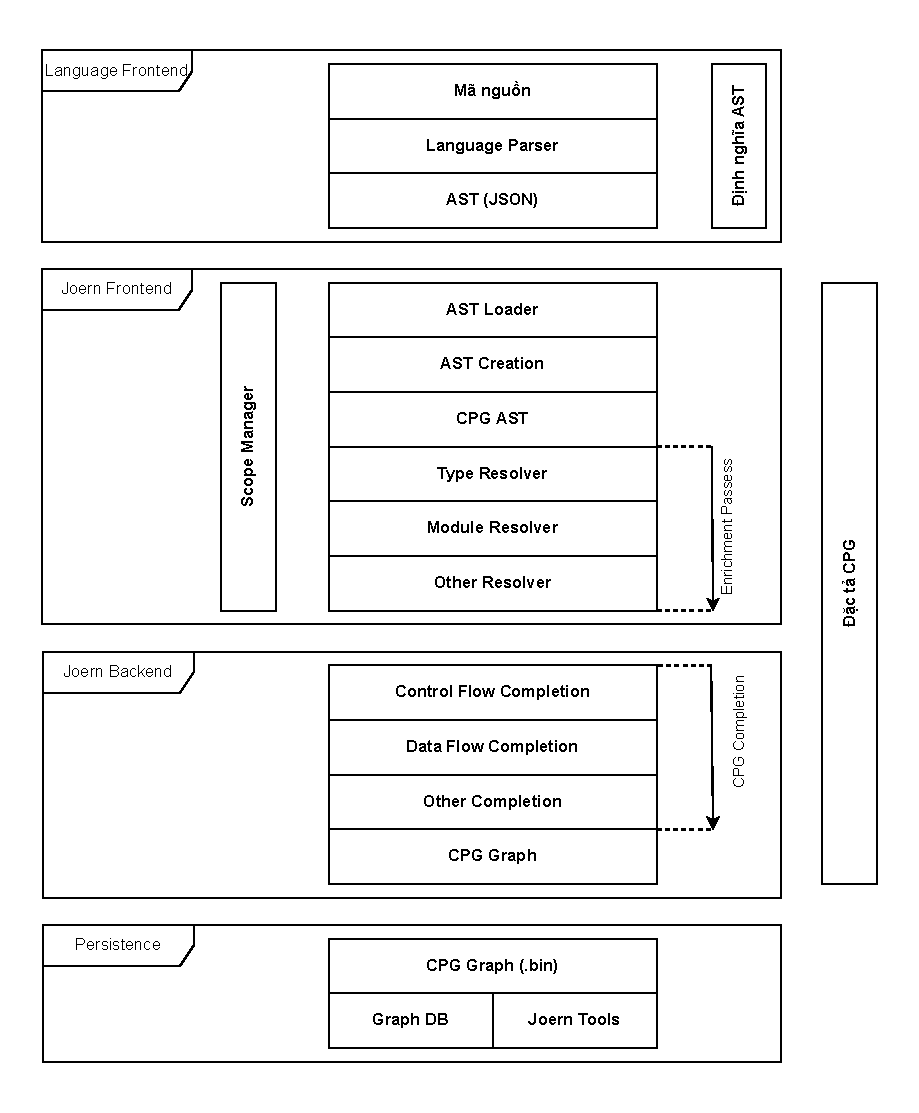
\includegraphics[width=1\columnwidth]{figures/c3/c3_arch.drawio.pdf}
	\centering
	\caption{Kiến trúc công cụ.}
	\label{img:c3_arch}
\end{figure}

\textbf{Joern Frontend.} Là nơi chính thực hiện các công việc chuyển đổi cây AST của một ngôn ngữ lập trình thành đồ thị CPG theo đặc tả CPG.
Đặc tả CPG sẽ được sử dụng xuyên suốt bởi Joern Frontend và Joern Backend.
Joern Frontend sẽ nhận dữ liệu từ Language Frontend dưới dạng JSON bằng bộ nạp AST.
Sau khi được nạp vào Joern Frontend dưới ngôn ngữ Scala, cây AST được chuyển đổi trước tiên thành cây CPG bằng bộ tạo AST CPG.
Bộ tạo AST CPG thực hiện ánh xạ mỗi một loại nút AST của ngôn ngữ sang một loại nút CPG tương ứng.
Bộ tạo AST CPG còn tạo các cạnh giữa các nút, giữa các nút có thể có nhiều cạnh, mỗi cạnh thể hiện một mối quan hệ giữa các nút.
Mặc định giữa các nút có mối quan hệ là cạnh \texttt{AST}.
Tùy vào thể loại nút thì sẽ có các cạnh thể hiện mối quan hệ khác, ví dụ nút \texttt{IF} sẽ có cạnh \texttt{CONDITION} nối với nút thể hiện biểu thức điều kiện.

\textbf{Bộ quản lý phạm vi.} Được sử dụng trong Joern Frontend để thực hiện quản lý phạm vi của các biến, hàm, khai báo.
Trong chương trình, một đơn vị thành phần sẽ có định danh riêng và hợp lệ trong một giới hạn nhất định.
Trong quá trình duyệt cây AST, bộ quản lý phạm vi sẽ kiểm soát thông tin về các định danh và phạm vi hoạt động của chúng.
Khi sử dụng một định danh hoặc khai báo một định danh mới, bộ quản lý phạm vi sẽ kiểm tra xem khai báo đó có hợp lệ trong phạm vi hay không.
Với bộ quản lý phạm vi ta có thể xác định được quan hệ giữa việc khai báo và sử dụng một biến, hàm hay đơn vị cấu trúc khác.
Từ đó có thể xác định được các cạnh giữa các nút trong cây CPG như cạnh \texttt{REF}, \texttt{REACHING DEFINITION}.
Các cạnh này sau sẽ được sử dụng để xây dựng đồ thị CFG và đồ thị PDG.

\textbf{Bộ giải.} Một phần của cây CPG đã được xây dựng bằng bộ tạo AST CPG kết hợp với bộ quản lý phạm vi.
Cây CPG sẽ tiếp tục được làm giàu thông tin bằng cách đi qua các bộ giải và được coi là đồ thị CPG chưa hoàn chỉnh.
Mỗi bộ giải sẽ bổ sung một lớp thông tin riêng biệt, ví dụ thông tin về kiểu dữ liệu, cấu trúc mô-đun, v.v.
Các lớp thông tin này hoàn toàn phụ thuộc vào ngữ cảnh của ngôn ngữ, do vậy số lượng bộ giải cũng sẽ không cố định.
Các bộ giải thao tác trên cây CPG nên có thể dùng chung cho nhiều ngôn ngữ, nhưng cũng có các bộ giải được xây dựng riêng cho một ngôn ngữ cụ thể.
Một bộ giải có thể phụ thuộc vào kết quả của bộ giải trước đó hoặc chạy độc lập nên thứ tự chạy các bộ giải có ảnh hưởng.
Ở đây, công cụ chỉ sử dụng 2 bộ giải là bộ giải kiểu dữ liệu và bộ giải mô-đun để xử lý hệ thống kiểu và hệ thống module của Rust, các bộ giải khác sẽ được xây dựng trong tương lai.
Sau khi chạy qua các bộ giải, cây CPG đã được bổ sung các lớp thông tin nhất định và đây cũng là công đoạn cuối cùng của Joern Frontend.

\textbf{Joern Backend.} Khi chuyển đổi một ngôn ngữ sang đồ thị CPG, người dùng phải tự thực hiện công đoạn Language Frontend và Joern Frontend để xây dựng đồ thị CPG.
Các thông tin có được từ hai bước trên sẽ được Joern Backend và các bộ hoàn thiện bên trong tận dụng để tự động xây dựng đồ thị CPG hoàn chỉnh.
Các nút, cạnh mới về luồng điều khiển, luồng dữ liệu sẽ được thêm vào và kết nối với các cạnh, nút đã tồn tại.
Không chỉ cung cấp lớp thông tin về luồng điều khiển và luồng dữ liệu, Joern Backend còn bổ sung các lớp thông tin đặc tả CPG riêng như \texttt{FileSystem}, \texttt{CallGraph}, \texttt{Shortcuts}, \texttt{TagsAndLocation}, và \texttt{Annotation} \cite{joernCodeProperty}.
Những lớp thông tin này giúp tăng cường khả năng truy vấn, phân tích, và phát hiện các vấn đề tiềm ẩn trong mã nguồn một cách hiệu quả hơn.
Kết quả cuối cùng của Joern Backend là một đồ thị CPG hoàn chỉnh, sẵn sàng phục vụ cho các bài toán như phân tích mã nguồn, phân tích bảo mật, hoặc trích xuất thông tin chuyên sâu.
Điều này cho phép người dùng tận dụng tối đa tiềm năng của Joern trong việc hiểu và cải thiện chất lượng mã nguồn.

\textbf{Persistence.} Đồ thị CPG có thể được lưu trữ bền vững dưới dạng tệp nhị phân.
Tệp này có thể tiếp tục được chuyển đổi thành kiểu dữ liệu tương thích với các cơ sở dữ liệu đồ thị như Neo4j để thực hiện các truy vấn phức tạp, hoặc sử dụng với các công cụ khác của Joern.
